\documentclass[11pt,a4paper]{article}
\usepackage{graphicx}

\begin{document}

% Title Page Contents
\title{Real Fantasy Adventure \\
Software Engineering Large Practical 14/15 \\
Report}
\author{Paul Scherer (s1206798)}
\maketitle
\newpage

\tableofcontents
\newpage

\section{Introduction}
This report describes the web application that was implemented as Part 2 of the Software Engineering Large Practical and make remarks based on proposal made as Part 1 of the practical. The purpose of the practical was to write a working web application that satisfied the following requirements.

\begin{itemize}
	\item A web application should be developed that doesn't need to be deployed globally but should be production ready
	\item The web application must run on DiCE and must be accessible via a browser available on DiCE
	\item There should be some notion of a user account
	\item Users should be ranked.
\end{itemize}

This has been the first time I have created a website, web application, or had anything to do with web development, moreover tackled a project of this size, and thus my inexperience had driven many of my design choices, planning, and implementation choices. Being wary of treading in unknown territory and using unfamiliar technologies, a lot of care was put in understanding and creating a maintainable project and following software engineering practices. This has resulted in a smaller implementation of the web application than originally set out in the proposal, however I feel proud of the things I have learnt and implemented to this point. Additionally, the project in its current state does satisfy, I believe, the requirements set out above.

The report will focus on the design, implementation, deficiencies and things I am particularly proud of having completed.

\subsection{Outline of Project}
The concept of the web application has not changed largely from Part 1. \textbf{Real Fantasy Adventure} is a web application that takes a user's real world activities (exercising, working, studying) and changes the stats of his/her \textit{Avatar} that exists in a fantasy world. In order to increase the avatar's stats, users log-in hours
of the real world activities they have performed through the interface provided in the web application. The system works largely on trust and user honesty in the name of role-play. Users compete against each other by gaining points within 3 categories: \textit{Professional}, \textit{Athletic}, and \textit{Academic}. Users are ranked by the amount of points within each of the categories and the best 5 are always displayed in the index page of the web application, naturally a full ranking is available as well. Users could set \textit{MyQuests} for themselves to further motivate themselves to complete goals they may have in the real world while also improving their avatar's stats (much like the motivation one gets by trying to increase the step count in a pedometer, by actually exercising and therefore satisfying two desires).

The largest change that has occurred since the proposal is the renaming of \textit{Quests} to \textit{MyQuests} as they were being set by the users, and the fact that these MyQuests do not award any rewarding bonus points, because they could be written by users for themselves. The entity \textit{Quest} still does exist but has changed to staff level creations, that could be taken on by avatars as official quests that would award extra points if achieved and only available depending on the level of the user's avatar. However while the Quest model and access/creation through staff has been implemented, its actual inclusion in this submission has been omitted due to implementation difficulties elaborated in another section.

\subsection{Quick Starting the Project}
Getting the project started has been described in the Quick Start section of the \verb|README.md| file in the top level of the practical. However it would be appreciated if more of the report is read to understand the project directory structure before the quick start guide us used to set up the project (though it is largely self-explanatory)

\subsection{Project Directory Structure}
The top level of the practical (and directory submitted) is the \verb|selpApp| folder which is a \textit{Git} directory that contains the django project \verb|rfa_website|, the \verb|README| file, the \verb|info| directory that holds the proposal and this report, and finally the \verb|requirements.txt| which lists the list of packages the project is dependent on for running on local host. The image below explains this better.

\begin{center}
\includegraphics[scale=0.5]{selpProjectStructure.png} \\
\end{center}

Global deployment would require more packages beyond those in the \verb|requirements.txt| to be installed as well as a few settings changed to increase the security of the web application. However this can be performed without altering the Real Fantasy Adventure web application itself (with the exception if a DBMS change is made), and installing packages and changing config files at the django project level can make deployment on a web hosting service such as \textit{Heroku} possible.

\subsubsection{The Django Project Directory}
The django project directory \verb|rfa_website| contains all of the code,the database (when created or the one submitted is used, both possibilities described in the quick start guide of the readme), and config files necessary to get the web application running. The \verb|real_fantasy_adventure_app| directory holds all of the code for the Real Fantasy Adventure web application. I had purposefully split the files in their respective directories, and logically decoupled functionality in the code (such as allowing the urls.py of the web application handle the url mapping within the application and only have the urls.py at website level shove the url mapping off to respective applications in order to decouple the code within the project as a whole as much as possible. I did this as it had been considered good practice in the official django documentation to make the application portable enough to be swapped between Django projects with minimal effort.


\section{Design Choices}
I have stuck to the design choices made in Part 1, with the exception of some of the packages that were installed in order to fulfill the requirements for a certain feature or make something easier. Most of these design choices were also made for the same reasons of inexperience. As I had expressed in the proposal I actually did spend 70\% of my time learning about web stacks, technologies, and idiomatic practices; and 30\% of my time on the implementation.

\subsection{Technologies}
\subsubsection{Python2.7.8}
I had decided on using Python2.7.8 as my main implementation language because I felt most comfortable using this language in this version from past experience. Additionally I had chosen python for its built in docstrings feature for easy documentation generation and ability to call this docstring simply by calling 'help' along with the class, function, method, or module. Python2.7.8 worked well together with \textit{virtualenv} on DiCE machines, whereas there was a bug in the version of virtualenv installed on DiCE in the creation of the virtual environment if initialized with the installed Python3.4 version, at least by the time of this writing (I realize there is a \textit{PyEnv} workaround that has been described in the informatics website, but didn't find this until later). Thus I have stuck to my decision to use Python2.7.8 despite the suggestion to use the newer version in the proposal feedback. However my code has been kept general enough so that even a web server running the project in Python3.x should theoretically work without problem save for a few lines that may need to be updated. However I think it still is important to be critical of using an older version when a newer one is present, and an older version always being prone support deprecation.

\subsubsection{Django 1.7}
I chose a heavier web development framework, Django1.7, because I saw it as an all-in-one package that contained a built-in web server, configuration files that were easy to edit, an integrated test suite that was easy to use, a large community of users for support, ORM functionality, and with the implementation language being python django appealed to me greatly as a newcomer to web development. Moreover the availability and ease of installing plug-ins to the framework was of great help to me in this practical. I spent a great amount of time making smaller applications (not relevant to this practical) in order to get used to the framework and initially found its strict Model-View-Template structure for data-driven applications a bit restrictive but over time have found its directed way of starting up applications helpful in getting applications on its feet quickly.

The ORM, and database migration management functionalities have made things much easier as curating a database manually would have taken me a lot of time to understand and perform. It is arguable that I may have learned even more about web technologies/development at a fundamental level had a taken a lighter framework such as \textit{flask} but I do not think I would have been able to create much of a project in the time I was given had I done so.

\subsubsection{HTML \& CSS with Django}
Having focused mainly on understanding the back-end handling of the web application with Django I ended up doing little in regards of making the web application pretty (though it would not be difficult to perform, for anyone who has a better design sense and HTML/CSS experience than I do). I have used html along with Django's templating system to create html pages with variable content pulled from the database to serve to the user instead of hard coded HTML. Additionally, using django's templating system I had all of the templates extend a base.html file so that the general look of the website can be changed wholly simply by changing this base HTML file and the CSS files referenced by it. I have used a CSS bundle provided by the \textit{Skeleton CSS Boiler Plate} (by Mr. Dave Gamache, under MIT License) project to style some aspects of the web application such as the buttons and forms, as I could not make it look good myself but was unwilling to use a larger package such as \textit{BootStrap} without fully utilizing and appreciating its strengths.
 
\subsubsection{SQLite3}
I have kept to using the standard database SQLite3 that is used by default for development in Django because I found it sufficient for my task and needs. Even in production I believe its use would be fine, as I don't expect many users in my application, and features involving concurrent updates and large scale calculations involving millions of rows is unlikely. Even so it would not be difficult to use another DBMS such as \textit{MySQL} or \textit{PostGreSQL} as these are supported by Django and can be used after changing the rfa\_website/settings.py DATABASES variable, as well as changing some model fields as necessary.

\subsection{Database Models}
As the models used in this application will be referenced in this report it may help to describe and display the relationships between the models. There are currently 3 implemented models in the \verb|models.py| with an additional standard User model used from \verb|django.contrib.auth.models| with the relationships described below.

\begin{center}
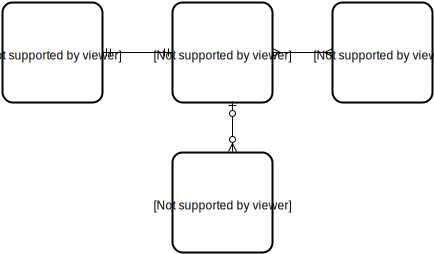
\includegraphics[scale=0.5]{selpModels.png} \\
\end{center}

Users and Avatars are tightly connected via a one to one relationship for the reason of this being part of the game setting, as well as functional as they together constitute an entity that I refer to as user/avatar in the report and in the source code. As one can see the Avatar is the central model in the application; as through the avatar the user can create MyQuests and take on Quests . Although the Quests feature is not part of the submitted project because of a deficiency described further below; as such the main models for the current web application are Users, Avatars, and MyQuests. MyQuests are said to 'belong' to an user/avatar and as such there is a optional one to many relationship between an Avatar and MyQuest instances.

\section{Development Process}
\subsection{Difficulties and Deficiencies}
As briefly mentioned before there were many difficulties i understanding and utilizing web development practices and web stacks due to inexperience and general ignorance, the lecture on webstacks definitely helped yet I had much to learn. A lot of time was spent trying to understand how web applications communicated with clients and URLs were handled. As a result much of what I had learned was not of much use in the end because I was researching and learning about the wrong things. In short the greatest difficulty was finding a foothold to start off of. This issue was resolved slowly simply by learning to look for the right information with more knowledge and trial and error. Due to my wariness I tried to follow good software engineering practices as early as possible as I began developing.

Approaching the problem in wrong way in the beginning, I had created the Quest model first instead of following my development schedule. I got very confused and focused on implementing a feature that was not even part of the requirements but rather an extra feature that was meant to be implemented once the minimum features and requirements were created and met respectively just to satisfy a curiosity. Next time I would look at the proposal ideas created initially, as some thought did go into it in the first place, and then compare it to the knowledge of the application/tools I had at the time of implementation begin.

\subsubsection{PEP Code Style}
I tried adopting (with varying success) PEP (Python Enchancement Protocols) practices in order to write idiomatic python code. In particular I tried to adhering to PEP8. I was greeted with little success in PEP8 as I constantly broke the 80 character guideline. Despite breaking these guidelines I tried my best to make my code as clear as possible, I believe this is especially evident in my tests and my population script.

\subsection{Things I am proud of}
\subsubsection{Usage of Git}
Knowing that I had potential to break a lot of things I resolved to use the Git VCS rigorously and correctly, and resolved to use branches wherever possible. In particular, this was useful when trying different authentication systems for the web application after having implemented user authentication. I had tried different 3rd party authentication packages such as django-allauth, and django-registration-redux both on different branches but was able to put these features aside safely after realising that they did not provide the expected improvement over what I had implemented/wanted and merged into the master branch before hand.

Moreover correctly using the add/reset commands after longer sessions allowed to me to make reasonable and rational commits. AdditionallyI strove for longer commit messages (though not always) so that I could pick up where I had left off if I were to stop working and pick up work several days later just by going through the commit log.

To improve usage I could have looked a bit more into the creation of git hooks or watchdog scripts that run the unit tests I had written as soon as a commit, push, or pull had been made.

\subsubsection{Issue Tracker}
Taking on the advice that "an issue tracker is \textit{never} overkill" from the feedback received I used a simple issue tracking system, in which I had kept a list of issue on sticky notes on a white board with priority levels on each of the issues. This allowed me to focus on important tasks/bugs that needed attention the most. Whenever an issue was fixed the [ISSUEFIX] or [BUGFIX] was used as a prefix to the commit message content, and the commit id placed on the issue to show that it has been dealt with. This system however is off-line and I should have an online solution such as the issue tracker provided by project management or SCM packages such as Trac. Unfortunately I was unable to resolve all issues that arose during development, some of which I have described as part of the functional deficiencies. 

\subsubsection{Documentation}
Having python as my main implementation language allowed me take advantage of Python's built in docstring abilities. As such I have included docstrings to each of the classes, functions, and methods I have written, but not at the module level, as I did not see this as necessary given how well defined and documented the standard modules utilised in django web applications are. However I must note I have no external documentation for developers nor a user manual (the web application is too simple at this point). However I would suggest the usage of the Sphinx Documentation Generator to create external documentation (by external I mean outside of the source code) of the docstrings I had written, and use the supported RestructuredText to create HTML friendly documentation that could be made available on the website for both developer documentation or user documentation. 

\subsubsection{Testing Strategy}
The tests are located in the \verb|../real_fantasy_adventure_app/tests.py|. There are 75 unit tests that can be run via the django test suite. Arguably there are cases I had not covered due to time constraints and I had overseen bugs in my views because I didn't write the view tests early and thought of all the possible cases for the views at the time of writing (described as functional deficiencies in the Implementation section), but I am proud of having understood the test structure and being able to find bugs in my code as I had written tests. As a result I have begun to appreciate the importance of tests much more in keeping code sane as it is refactored or changed and as a way of validating intended behaviour. Using the \textit{coverage} package and running the commands: (this requires that the project already be set up or be in a state able to run these tests as described in the readme file)

\begin{verbatim}
	coverage run --source='.' manage.py test real_fantasy_adventure_app
	coverage report
\end{verbatim}

in the \verb|selpApp/rfa_website/| directory gave me 91\% statement coverage as shown below.

\begin{center}
\includegraphics[scale=0.5]{selpTestCoverage.png} \\
\end{center}

In addition to the automated tests, I believe a manual testing procedure would be helpful to ensure correct/expected display of items in the screen web application. While these would not be carried out with the regularity of the automated tests being run each time development starts, ends, commits are made, or another test is added; the manual tests could be run each time a release would be scheduled iteratively (if an agile methodology like \textit{Scrum} were followed with its regular short releases). To this end a database population script had been created known as \verb|selpApp/rfa_website/populate.py| had been provided to quickly create a set amount of users, avatars, and myquests (default 100 test users/avatars, and 3 MyQuests for each avatar). If a manual test is difficult, browser tests could be carried out by specified testing frameworks for this particular purpose like \textit{Selenium}.

\subsubsection{Idiomatic Style}
As described in the 'PEP Code Style' section above I had some trouble writing code in the PEP style, I tried to follow good coding practices by making my signatures as explicit and self explanatory as possible. As mentioned this is particularly evident in my \verb|../real_fantasy_adventure_app/tests.py| tests file, or in models file.

While this is a smaller note, I had originally hard-coded each of the HTML files that the view had returned when a request had been made. However I had learned of using django's templating engine and HTML file extension to create a unified look, and felt this was another example of following idiomatic practices in django (and other web frameworks at large).

\section{Implementation}
\subsection{Requirements}
In this section the implementation of the latter two of the four basic requirements outlined above are discussed. In the omitted first two of the four basic requirements, the first is something I aspired to satsify (though my word wouldn't be convincing enough) and the second one has been satisfied, by having developed and tested (both through automated and manual means) most of my application on DiCE.

\subsubsection{User Accounts \& Authentication}
Using Django's included User model and authentication system I had created a rudimentary user authentication using django's auth package. Coupled with users one to one relationship to avatars, the avatar profiles satisfy the notion of the user accounts, that can be ranked.

\subsubsection{Ranking System}
In its current state the users are ranked by the amount of points their avatars have earned in each of the categories: Professional, Athletic, and Academic. A full rankings page showing all of the avatars ranked by decreasing order of their respective categories is available from the index (or home) page. In fact the index page shows the current top 5 avatars in each of the categories. This is currently lacking the total points ranking because I found it troublesome to rank the models according to a function return rather than a attribute, however, this should be easy to fix, but haven't in order to focus on another program and to write tests. Nonetheless I believe even in its most rudimentary state it is in now, I believe it satisfies the user ranking requirement, and has potential to be expanded greatly with more categories and filtering features.

\subsection{Current Functional Deficiencies}
As a result of underestimating the project and making mistakes in the learning phase, there are many features I would have liked to implement as well as a few functional deficiencies (as well as bugs) in what has been implemented and this section is dedicated to the latter.

\subsubsection{Quest Model}
The Quest model that has been implemented in the beginning of the development process has been pushed to the back and in its current state has not been included in the main function of the web application (as planned in development stage 5 [extra] of the proposal). The main reason for this is the unclear understanding logically of how avatars can take on Quests. Clearly Avatars share a many to many relationship but beyond this I don't see how users can 'accept' or 'clear' Quests. A boolean variable in Quests could help. This is a frustrating deficiency as considerable work and thought has gone to this feature already, with staff being able to write Quests in the admin view with markdown support and so forth. I mark this as a design and implementation deficiency that has to be rethought, but should be implementable with some more time.

\subsubsection{StatChange lacks Value Check}
Currently the user can add any number of points to log in to their hours, as it was undecided at a business logic level to allow or disallow more than 24 points being added total to an avatar a day. If it were to disallow the addition of more than 24 points to the avatar, I would have used a cookie that is checked by the server when the user calls the statChange view. Thus at the moment any number of points (even negatives) are allowed because game logic for section hasn't been decided upon (but the implementation for any of the cases is clear).


\end{document}
